\documentclass[]{article}

% Imported Packages
%------------------------------------------------------------------------------
\usepackage{amssymb}
\usepackage{amstext}
\usepackage{amsthm}
\usepackage{amsmath}
\usepackage{enumerate}
\usepackage{fancyhdr}
\usepackage[margin=1in]{geometry}
\usepackage{graphicx}
%\usepackage{extarrows}
%\usepackage{setspace}
%------------------------------------------------------------------------------

% Header and Footer
%------------------------------------------------------------------------------
\pagestyle{plain}  
\renewcommand\headrulewidth{0.4pt}                                      
\renewcommand\footrulewidth{0.4pt}                                    
%------------------------------------------------------------------------------

% Title Details
%------------------------------------------------------------------------------
\title{Deliverable \#2 Template}
\author{SE 3A04: Software Design II -- Large System Design}
\date{}                               
%------------------------------------------------------------------------------

% Document
%------------------------------------------------------------------------------
\begin{document}

\maketitle	
\noindent{\bf Tutorial Number:} T01\\
{\bf Group Number:} G6 \\
{\bf Group Members:} 
\begin{itemize}
	\item Jane Klavir
	\item Nathan Luong
	\item Areez Visram
	\item Jennifer Ye
\end{itemize}

\section*{IMPORTANT NOTES}
\begin{itemize}
	%	\item You do \underline{NOT} need to provide a text explanation of each diagram; the diagram should speak for itself
	\item Please document any non-standard notations that you may have used
	\begin{itemize}
		\item \emph{Rule of Thumb}: if you feel there is any doubt surrounding the meaning of your notations, document them
	\end{itemize}
	\item Some diagrams may be difficult to fit into one page
	\begin{itemize}
		\item Ensure that the text is readable when printed, or when viewed at 100\% on a regular laptop-sized screen.
		\item If you need to break a diagram onto multiple pages, please adopt a system of doing so and thoroughly explain how it can be reconnected from one page to the next; if you are unsure about this, please ask about it
	\end{itemize}
	\item Please submit the latest version of Deliverable 1 with Deliverable 2
	\begin{itemize}
		\item Indicate any changes you made.
	\end{itemize}
	\item If you do \underline{NOT} have a Division of Labour sheet, your deliverable will \underline{NOT} be marked
\end{itemize}

\newpage
\section{Introduction}
\label{sec:introduction}
% Begin Section

This section should provide an brief overview of the entire document.

\subsection{Purpose}
\label{sub:purpose}
% Begin SubSection
State the purpose and intended audience for the document.
% End SubSection

\subsection{System Description}
\label{sub:system_description}
% Begin SubSection
Give a brief description of the system. This could be a paragraph or two to give some context to this document.

% End SubSection

\subsection{Overview}
\label{sub:overview}
% Begin SubSection
Describe what the rest of the document contains and explain how the document is organised (e.g. "In Section 2 we discuss...in Section 3...").

% End SubSection

% End Section

\section{Analysis Class Diagram}
\label{sec:analysis_class_diagram}
% Begin Section
This section should provide an analysis class diagram for your application.
% End Section


\section{Architectural Design}
\label{sec:architectural_design}
% Begin Section
This section should provide an overview of the overall architectural design of your application. Your overall architecture should show the division of the system into subsystems with high cohesion and low coupling.

\subsection{System Architecture}
\label{sub:system_architecture}
% Begin SubSection
\begin{itemize}
	\item Identify and explain the overall architecture of your system
	\item Be sure to clearly state the name of the architecture you used (this is the name of the architectural pattern, not the name of your system)
	\item Provide the reasoning and justification of the choice of architecture
	\item Provide a structural architecture diagram showing the relationship among the subsystems (if appropriate)
	\item List any design alternatives you considered, but eliminated (and explain why you eliminated them)
\end{itemize}
\subsubsection{Overall Architecture and Justification}
\label{subsub:overall_architecture}
% Begin SubSubSection
The overall architecture of the system is the Model-View-Controller (MVC) architecture, which is an interaction 
oriented architecture. The MVC architecture is the architecture that best fits the system that we are designing. The MVC style is best suited for 
interactive applications which contain multiple views for various data models. The application being implemented is heavily focused on the UI 
on the mobile app, and so an architecture style that allows for easy display of data into a UI view is suitable. Furthermore, our system contains multiple data models, for example, models for Users, 
Rides, Prompts and multiple pages/views across the application will interact with these data models. Furthermore, the MVC architecture is suitable for 
applications which are prone to frequent data changes. Our system is most definitely prone to frequent data changes, as rides are constantly being offered, 
arriving, and starting, which means the Rides model will be constantly updated and written to. Finally, the MVC architecture will allow us to separate the 
various logic functions into separate controllers. The architecture will allow for clear division of logic between controllers, which will make it easier 
to extend and modify the system. For example, we would have a UserController to handle user operations, a RidesController to handle ride operations and various 
other controllers to control the logic of other parts of the application. Given these benefits and the functionality of the system, we have chosen to implement 
the MVC architecture style for the main system.

\subsubsection{Subsystem Architectures and Justification}
Another architecture style will also be used for the various subsystems of our application. One of the subsystems within the main system is the Dispatcher 
subsystem, which is responsible for storing all information on taxis and carpool offerings, as well as deciding how to match carpool offers with 
requests that come in. The repository architecture style is best suited for systems (in this case a subsystem) in which a central data store stores information 
and various agents communicate with it. This architecture style fits the Dispatcher subsystem because the Dispatcher will contain a central data store which 
will store all the information about carpools. The data store will be passive, it will be like a database which just stores information and can be read from. 
The various agents for the repository will be the users who are requesting and offering carpools. These agents are active, as they drive the flow of the 
subsystem by sending carpool requests and offering carpools. The agents do not communicate directly with each other, they communicate via the data store by 
sending requests to the data store, and the data store facilitates the requests and decides appropriate matches. Given this, the repository architecture style 
is the most suitable for the Dispatcher subsystem.
% End SubSubSection

% Begin SubSubSection
\subsubsection{Structural Architecture Diagram}
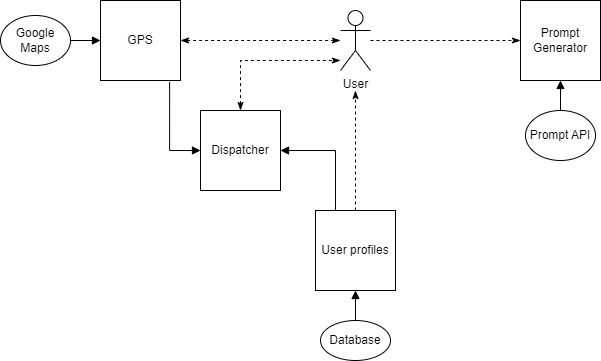
\includegraphics[scale = 0.7]{Graphics/subsystems_diagram_3.1.png}
% End SubSubSection

% Begin SubSubSection
\subsubsection{Design Alternatives Considered}
One design alternative for the main architecture that was considered was the Repository architectural style, which is a data centered architecture. We envisioned the system having a 
central passive database repository, with multiple active agents communicating with the data store. The agents were envisioned to be the different parts of 
the system, such as a user agent, a rides agent, a prompts agent, and then a dispatcher, all which communicated with the central data store. However, this design 
was not chosen because the system that is being built is a single mobile application connected to a database. The system does not involve multiple agents which 
must communicate with a central data store. If there were multiple applications that needed to communicate, this architecture style would be more applicable. However, 
is is a single application and the different parts of it can be represented using controllers within the architecture rather than external agents, so this design 
was not chosen. \\

\noindent The second design alternative for the main architecture that was considered was the Presentation-Abstraction-Control (PAC) architecture, which is also 
an interaction oriented architecture. Both MVC (the architecture that was chosen) and PAC could work for this system, but we ultimately chose MVC over PAC for 
various reasons. PAC was not chosen because PAC is more useful in complex applications, which require a hierarchical layering of agents. Our system is not complex, 
it is a single application that communicates with a database. In PAC, the only communication that can occur is between agents, and in our system, we would not 
have enough agents to justify having communication only between them. This would only add complexity. Furthermore, PAC is more useful for concurrent systems, which 
our app does not need to be to fulfill its requirements. Finally, PAC is less publicized and less widely used, and so for a somewhat inexperienced development team, MVC 
is a better choice as there are more resources, information and examples available to help in the design.
% End SubSubSection
% End SubSection

\subsection{Subsystems}
\label{sub:subsystems}
% Begin SubSection
The first subsystem is the dispatcher. The dispatcher is a data store for all communications within our system. It acts as the data store in the repository architecture which is the architecture style that this subsystem follows. The dispatcher has several purposes. The first is to store information about active taxis in the fleet. It also stores information about user offers and requests. Subsequently, the dispatcher suggests “offerers” to “requesters”, and once a “requester” requests to join the “offerer’s” taxi, the dispatcher must also display an updated fare to the “offerer” so that they can make an informed decision. This match-making process is another fundamental purpose of the dispatcher.
\\\\
The next subsystem is the user profile subsystem, that handles tasks having to do with the processing and storage of user profiles. One main purpose of this subsystem is to facilitate the registration of new users. It records their information and remembers it in a database. Furthermore, another purpose is to allow registered users to make updates to their profile. When users edit their profiles, the user profile subsystem must make the necessary updates to the database so that all the information is up to date. Additionally, this subsystem allows registered users to delete their profiles, thenceforth these profiles are removed from the database.
\\\\
Another subsystem is the GPS. The purpose of this subsystem is to allow users to track the route of their taxi. Also, it uses the carpoolers’ locations to determine distances between carpoolers. The GPS subsystem requires interfacing with Google Maps.
\\\\
The final subsystem is the prompt generator. This subsystem executes our additional innovative feature, which is allowing carpoolers to socialize through a series interesting prompts. The prompt generator must also implement an API to fulfill its purpose of coming up with prompts.
\\\\
The subsystems interact with one another when it comes to the match-making procedure described in the dispatcher subsystem. The dispatcher is at the centre of it all, and for it to perform its role, it uses the user profile and GPS subsystems to obtain critical information. First, the user profiles subsystem provides data on users’ social preferences, which helps the dispatcher predict user compatibility. Then, the GPS subsystem returns distances between the taxi and potential matches, which the dispatcher uses in showing trip conditions (estimated fare, time, and distance). Ultimately, this relationship is one in which the dispatcher is the central unit, and it uses the other subsystems to get the necessary parameters for its algorithm.
\\
% End SubSection

% End Section
	
\section{Class Responsibility Collaboration (CRC) Cards}
\label{sec:class_responsibility_collaboration_crc_cards}
% Begin Section
This section should contain all of your CRC cards.

\begin{itemize}
	\item Provide a CRC Card for each identified class
	\item Please use the format outlined in tutorial, i.e., 
	\begin{table}[ht]
		\centering
		\begin{tabular}{|p{5cm}|p{5cm}|}
		\hline 
		 \multicolumn{2}{|l|}{\textbf{Class Name:}} \\
		\hline
		\textbf{Responsibility:} & \textbf{Collaborators:} \\
		\hline
		\vspace{1in} & \\
		\hline
		\end{tabular}
	\end{table}
	
\end{itemize}
% End Section

\appendix
\section{Division of Labour}
\label{sec:division_of_labour}
% Begin Section
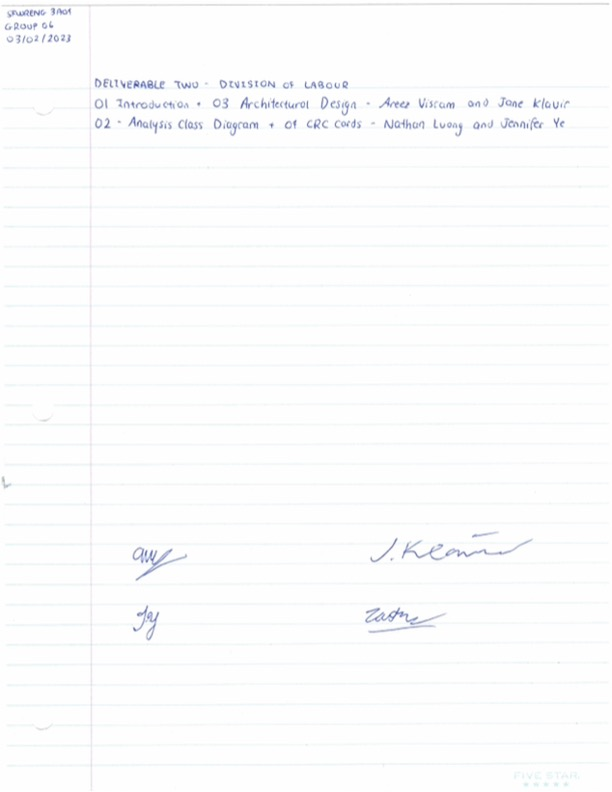
\includegraphics[scale = 0.6]{Graphics/DivisionOfLabour.jpg}
% End Section


\end{document}
%------------------------------------------------------------------------------